\documentclass[aspectratio=169]{beamer}
\usetheme{Madrid}
\usecolortheme{default}
\usepackage[utf8]{inputenc}
\usepackage[T5]{fontenc}
\usepackage{graphicx}
\usepackage{hyperref}
\usepackage{booktabs}
\usepackage{amsmath}
\usepackage{listings}
\usepackage{color}

\definecolor{codegreen}{rgb}{0,0.6,0}
\definecolor{codegray}{rgb}{0.5,0.5,0.5}
\definecolor{codepurple}{rgb}{0.58,0,0.82}
\definecolor{backcolour}{rgb}{0.95,0.95,0.92}

\lstdefinestyle{mystyle}{
    backgroundcolor=\color{backcolour},   
    commentstyle=\color{codegreen},
    keywordstyle=\color{magenta},
    numberstyle=\tiny\color{codegray},
    stringstyle=\color{codepurple},
    basicstyle=\ttfamily\scriptsize,
    breakatwhitespace=false,         
    breaklines=true,                 
    captionpos=b,                    
    keepspaces=true,                 
    numbers=left,                    
    numbersep=5pt,                  
    showspaces=false,                
    showstringspaces=false,
    showtabs=false,                  
    tabsize=2
}
\lstset{style=mystyle}

\setbeamertemplate{caption}[numbered]
\renewcommand{\figurename}{Hình}
\renewcommand{\thefigure}{16.\arabic{figure}}

\title[Chương 16: Sinh văn bản]{Học Sâu (Deep Learning) \\ \vspace{0.5cm} \Large Chương 16: Sinh văn bản \& Kỷ nguyên AI Tạo sinh}
\author{Đại học Đông Á}
\date{\today}

\begin{document}

\begin{frame}
    \titlepage
\end{frame}

\begin{frame}{Nội dung chương}
    \tableofcontents
\end{frame}

\section{1. Kỷ nguyên AI Tạo sinh \& Lịch sử phát triển}

\begin{frame}{Trí tuệ Nhân tạo Tạo sinh là gì?}
    \begin{itemize}
        \item Khác biệt với AI Phân loại (Classification) dùng để nhận diện dữ liệu, \textbf{Generative AI} được thiết kế để \textbf{tạo ra nội dung hoàn toàn mới} (Văn bản, Hình ảnh, Âm thanh, Code).
        \item AI tạo sinh hoạt động bằng cách học các mẫu (patterns) và cấu trúc thống kê ẩn (Latent space) từ lượng dữ liệu khổng lồ của con người.
        \item Sau đó, nó thực hiện một phép "lấy mẫu" (Sampling) từ không gian tiềm ẩn đó để tạo ra các tác phẩm có đặc điểm tương tự dữ liệu huấn luyện.
    \end{itemize}
\end{frame}

\begin{frame}{Sự kết hợp giữa AI và Nghệ thuật}
    \begin{columns}
        \column{0.5\textwidth}
        \begin{itemize}
            \item AI không "cướp" đi sự sáng tạo, mà đóng vai trò như một chiếc bút vẽ quyền năng (Augmented Intelligence).
            \item Midjourney, DALL-E, hay Stable Diffusion cho phép tạo ra các tác phẩm nghệ thuật phức tạp chỉ bằng ngôn ngữ (Prompt engineering).
            \item Lấy mẫu không gian tiềm ẩn thiết lập một phương tiện biểu đạt thuần túy mới, tách nghệ thuật ra khỏi thủ công.
        \end{itemize}
        
        \column{0.5\textwidth}
        \begin{figure}
            \centering
            \includegraphics[width=\textwidth,height=0.6\textheight,keepaspectratio]{../../images/ch16/keras-midjourney-image.edfbf674.png}
            \caption{Hình ảnh tạo ra từ Midjourney bằng văn bản}
        \end{figure}
    \end{columns}
\end{frame}

\begin{frame}{Sơ lược về lịch sử tạo trình tự (Sequence Generation)}
    \begin{itemize}
        \item Trước đây, tạo chuỗi văn bản là một chủ đề phụ. Năm 1997, mạng LSTM ra đời và năm 2002 được áp dụng vào sản xuất âm nhạc.
        \item Năm 2013, Alex Graves dùng mạng lặp lại (RNN) để tạo ra chữ viết tay giống con người.
        \item \textbf{Bước ngoặt 2018:} OpenAI kết hợp Đào tạo trước không giám sát (Unsupervised Pretraining), Kiến trúc Transformer và Dữ liệu khổng lồ để tạo ra \textbf{GPT} (Generative Pretrained Transformer).
    \end{itemize}
\end{frame}

\begin{frame}{Sự phát triển từ GPT-1 đến GPT-3}
    \begin{itemize}
        \item \textbf{GPT-1 (2018):} 117 triệu tham số, huấn luyện trên 1 tỷ token. Mục tiêu: đoán từ tiếp theo. Cần tinh chỉnh để làm các tác vụ cụ thể.
        \item \textbf{GPT-2 (2019):} 1.5 tỷ tham số, 10 tỷ token. Phát hiện ra khả năng \textbf{Học trong vài lần (Few-shot learning)}, không cần tinh chỉnh lại trọng số.
        \item \textbf{GPT-3 (2020):} 175 tỷ tham số, 500 tỷ token. Không cần ví dụ, chỉ cần cung cấp mô tả văn bản đơn giản (Zero-shot learning) là có kết quả chất lượng.
    \end{itemize}
\end{frame}

\begin{frame}{Sự bùng nổ của Large Language Models (LLMs)}
    \begin{columns}
        \column{0.5\textwidth}
        \begin{itemize}
            \item Nhờ kiến trúc Transformer, khả năng mở rộng (Scale-up) của mô hình ngôn ngữ bùng nổ dữ dội.
            \item Các tập dữ liệu huấn luyện mở rộng từ hàng chục Gigabyte (BooksCorpus) lên đến hàng Terabyte.
            \item Kích thước tham số của mô hình cũng vượt qua mốc 100 tỷ, thậm chí nghìn tỷ.
        \end{itemize}
        
        \column{0.5\textwidth}
        \begin{figure}
            \centering
            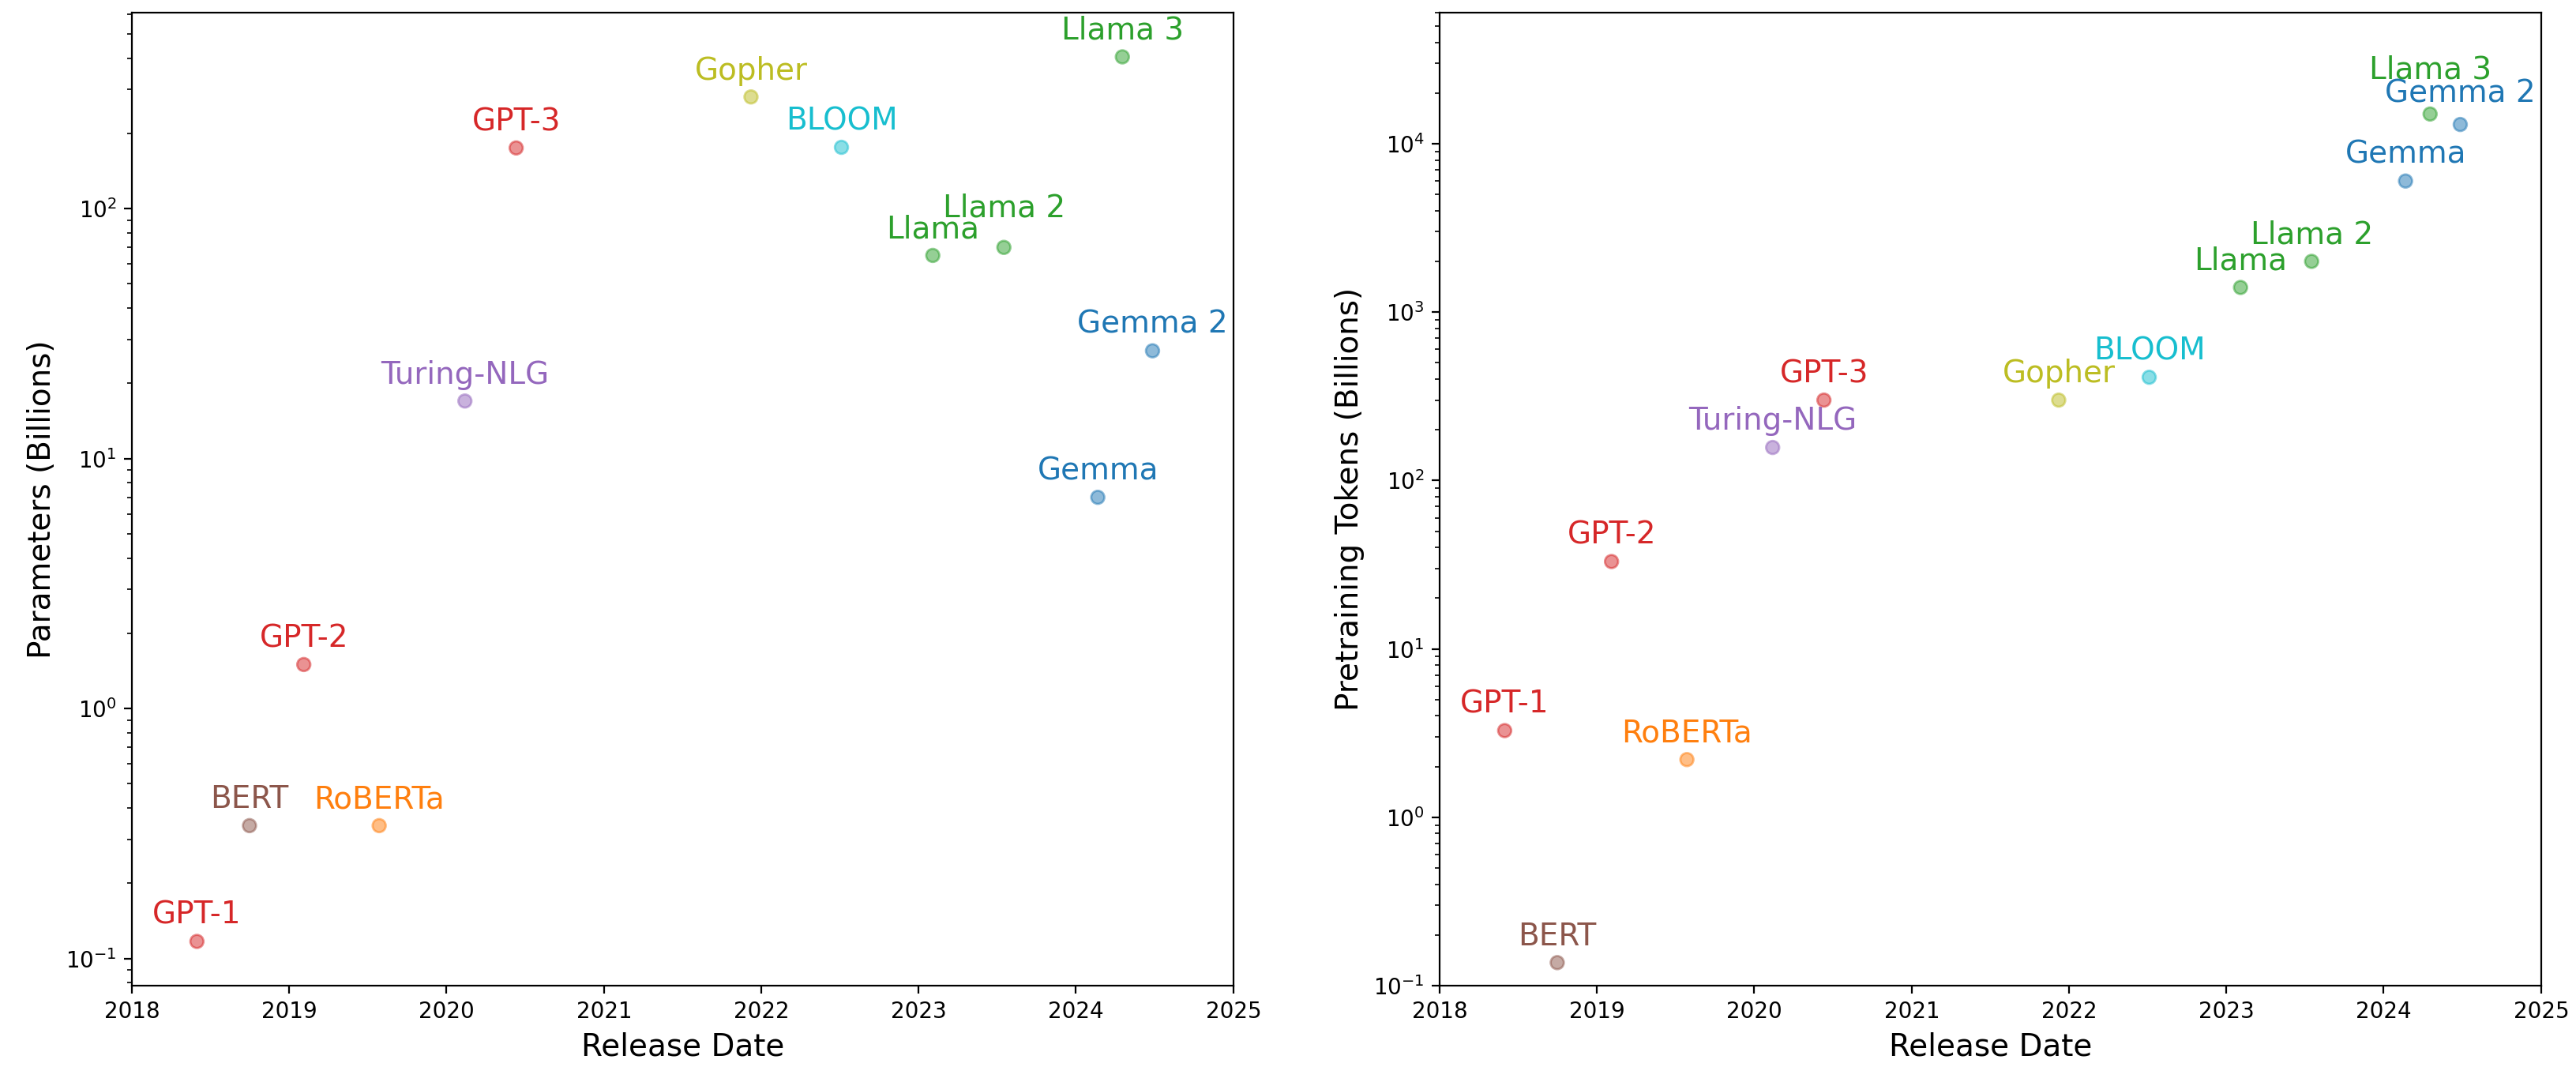
\includegraphics[width=\textwidth,height=0.6\textheight,keepaspectratio]{../../images/ch16/llm-sizes.34d71a34.png}
            \caption{Sự gia tăng kích thước của LLM theo thời gian}
        \end{figure}
    \end{columns}
\end{frame}

\section{2. Đào tạo mô hình mini-GPT từ đầu}

\begin{frame}{Dữ liệu đào tạo: Tập C4 và Tokenization}
    \begin{itemize}
        \item \textbf{Colossal Clean Crawled Corpus (C4):} Tập dữ liệu văn bản thu thập từ web khổng lồ do Google phát hành.
        \item Để huấn luyện, ta dùng \textbf{SentencePiece} để mã hóa văn bản thành các token số nguyên (Subword tokenization).
        \item \textbf{Ranh giới tài liệu:} Sử dụng token đặc biệt \texttt{<|endoftext|>} để phân tách giữa các tài liệu khác biệt trên web.
    \end{itemize}
\end{frame}

\begin{frame}[fragile]{Xây dựng Pipeline dữ liệu}
\begin{lstlisting}[language=Python]
import tensorflow as tf

# Tokenize and format the dataset using tf.data
def read_file(filename):
    ds = tf.data.TextLineDataset(filename)
    ds = ds.map(lambda x: tf.strings.regex_replace(x, r"\\n", "\n"))
    ds = ds.map(tokenizer, num_parallel_calls=8)
    # Add end of text token
    return ds.map(lambda x: tf.concat([x, suffix], -1))

ds = ds.interleave(read_file, cycle_length=32)
ds = ds.rebatch(sequence_length + 1, drop_remainder=True)
# Split to (inputs, labels) offset by 1
ds = ds.map(lambda x: (x[:-1], x[1:])) 
\end{lstlisting}
\end{frame}

\begin{frame}{Kiến trúc Transformer Decoder-only}
    \begin{itemize}
        \item Mô hình GPT chỉ sử dụng phần \textbf{Decoder} của Transformer.
        \item Lớp \textbf{Cross-attention} (chú ý chéo) bị loại bỏ do không có phần Encoder.
        \item Thông tin truyền một chiều: Các token không thể nhìn thấy token tương lai nhờ vào Causal Masking (Mặt nạ nhân quả).
        \item Câu hỏi và câu trả lời được nối chung thành một chuỗi duy nhất để đưa vào mạng.
    \end{itemize}
\end{frame}

\begin{frame}{Kỹ thuật Nhúng nghịch đảo (Reversible Embedding)}
    \begin{itemize}
        \item \textbf{Vấn đề:} Trọng số lớn nhất của mô hình là lớp Embedding đầu vào và lớp Projection đầu ra. Kích thước \texttt{vocab\_size} $\times$ \texttt{hidden\_dim}.
        \item \textbf{Giải pháp:} Liên kết hai ma trận trọng số này lại với nhau (Weight Tying).
        \item Đầu ra cuối cùng là phép nhân ma trận trạng thái ẩn với \textbf{ma trận chuyển vị} của lớp Token Embedding ban đầu, tiết kiệm đáng kể tham số cho mô hình.
    \end{itemize}
\end{frame}

\begin{frame}{Learning Rate Warmup trong Huấn luyện}
    \begin{columns}
        \column{0.5\textwidth}
        \begin{itemize}
            \item Mô hình Transformer cực kỳ nhạy cảm ở giai đoạn đầu do khởi tạo ngẫu nhiên.
            \item Nếu dùng Tốc độ học (Learning Rate) quá lớn ngay từ đầu, gradient sẽ phát nổ, mô hình không hội tụ.
            \item \textbf{Warmup:} Bắt đầu LR ở 0, tăng dần tuyến tính qua hàng nghìn bước đầu tiên (Warmup phase) để làm nóng ổn định.
        \end{itemize}
        
        \column{0.5\textwidth}
        \begin{figure}
            \centering
            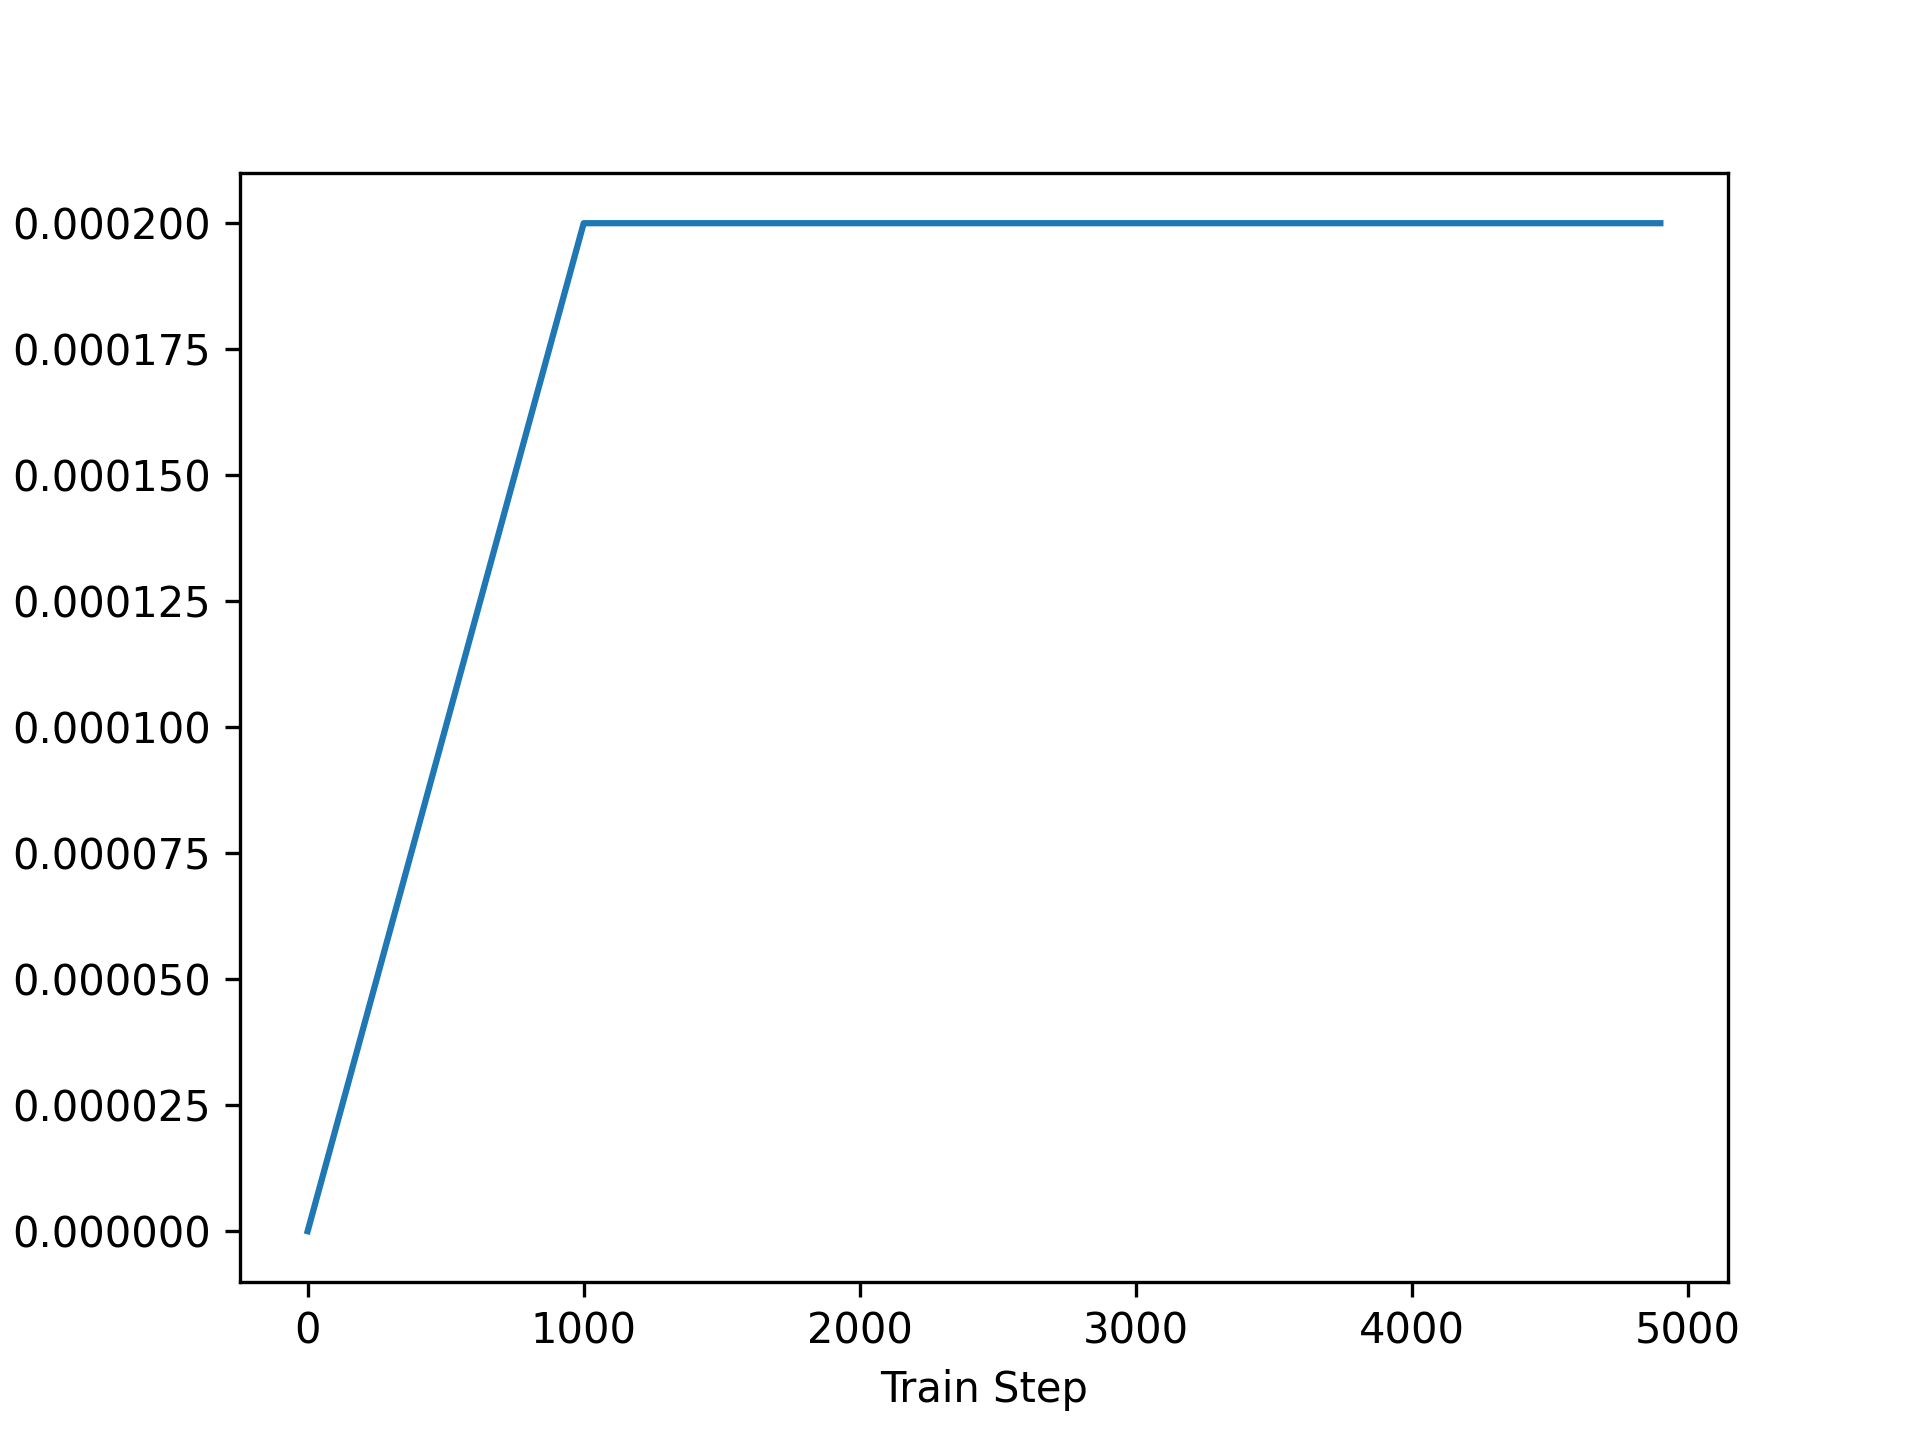
\includegraphics[width=\textwidth,height=0.6\textheight,keepaspectratio]{../../images/ch16/learning-rate-warmup.e99ec2a4.png}
            \caption{Đồ thị Learning Rate Warmup}
        \end{figure}
    \end{columns}
\end{frame}

\begin{frame}{Giải mã Sáng tạo \& Vấn đề biên dịch (Compilation)}
    \begin{itemize}
        \item Quá trình sinh văn bản lặp lại từng token một. Mỗi khi có token mới, chuỗi càng dài ra.
        \item Việc liên tục thay đổi kích thước mảng đầu vào sẽ khiến TensorFlow/JAX phải \textbf{biên dịch lại hàm tính toán} (re-compile) liên tục, tốc độ cực chậm.
        \item \textbf{Padding:} Cố định độ dài chuỗi đầu vào ngay từ đầu để tránh biên dịch lại đồ thị tính toán.
        \item Quá trình dự đoán trả về \textbf{Logits} (xác suất log chưa chuẩn hóa) giúp xử lý các phép lấy mẫu dễ dàng.
    \end{itemize}
\end{frame}

\begin{frame}{Tối ưu Giải mã với Key-Value Caching}
    \begin{itemize}
        \item Trong vòng lặp sinh từ, chỉ có token cuối cùng là mới. Việc tính toán lại toàn bộ lớp Attention cho các token trước đó là vô cùng lãng phí.
        \item Vì \textbf{Query, Key, Value} của các token quá khứ không hề thay đổi.
        \item \textbf{Cơ chế KV Cache:} Lưu trữ lại mảng Key và Value ở mỗi lớp Transformer. Ở bước sinh tiếp theo, mô hình chỉ tính Q, K, V cho token hiện tại và chấm (dot-product) với bộ nhớ đệm KV có sẵn.
        \item Kỹ thuật này giúp tăng tốc độ sinh văn bản lên hàng nghìn lần!
    \end{itemize}
\end{frame}

\section{3. Chiến lược lấy mẫu (Sampling Strategies)}

\begin{frame}{Làm sao AI có tính "Sáng tạo"?}
    \begin{itemize}
        \item Bản chất của LLM là xuất ra một mảng Xác suất (Probability Distribution) cho hàng chục nghìn từ vựng ở vị trí tiếp theo.
        \item Nếu luôn chọn từ có xác suất cao nhất (\textbf{Greedy Search}), mô hình dễ rơi vào vòng lặp rập khuôn vô tận (ví dụ: lặp đi lặp lại chữ "the").
        \item \textbf{Giải pháp:} Đưa sự \textbf{Ngẫu nhiên} vào bằng cách lấy mẫu (sampling) trực tiếp từ phân phối xác suất.
    \end{itemize}
\end{frame}

\begin{frame}{Kỹ thuật Nhiệt độ (Temperature Sampling)}
    \begin{itemize}
        \item Nhiệt độ $T$ là một siêu tham số điều khiển mức độ "Sáng tạo".
        \item \textbf{Khi $T < 1$ (VD: $0.2$):} Các logit lớn trở nên lớn hơn, xác suất tập trung vào các từ chắc chắn (Mô hình an toàn, bảo thủ).
        \item \textbf{Khi $T > 1$ (VD: $1.5$):} Phân bố xác suất bị san bằng, mô hình dám chọn những từ rất lạ (Mô hình sáng tạo, phá cách).
        \item \textbf{Khi $T \to 0$:} Trở thành Greedy Search thuần túy.
    \end{itemize}
\end{frame}

\begin{frame}{Kỹ thuật Top-K và Top-p}
    \begin{columns}
        \column{0.5\textwidth}
        \begin{itemize}
            \item \textbf{Top-K:} Lọc ra $K$ ứng viên có xác suất cao nhất. Loại bỏ hoàn toàn phần dư, lấy mẫu ngẫu nhiên trong nhóm K từ.
            \item \textbf{Top-p (Nucleus):} Lọc ra một nhóm từ sao cho tổng xác suất cộng dồn vừa chạm ngưỡng $p$ (VD: $0.9$).
            \item Top-p linh hoạt hơn Top-K vì số lượng từ ứng viên tự co giãn tùy vào độ chắc chắn của mô hình.
        \end{itemize}
        
        \column{0.5\textwidth}
        \begin{figure}
            \centering
            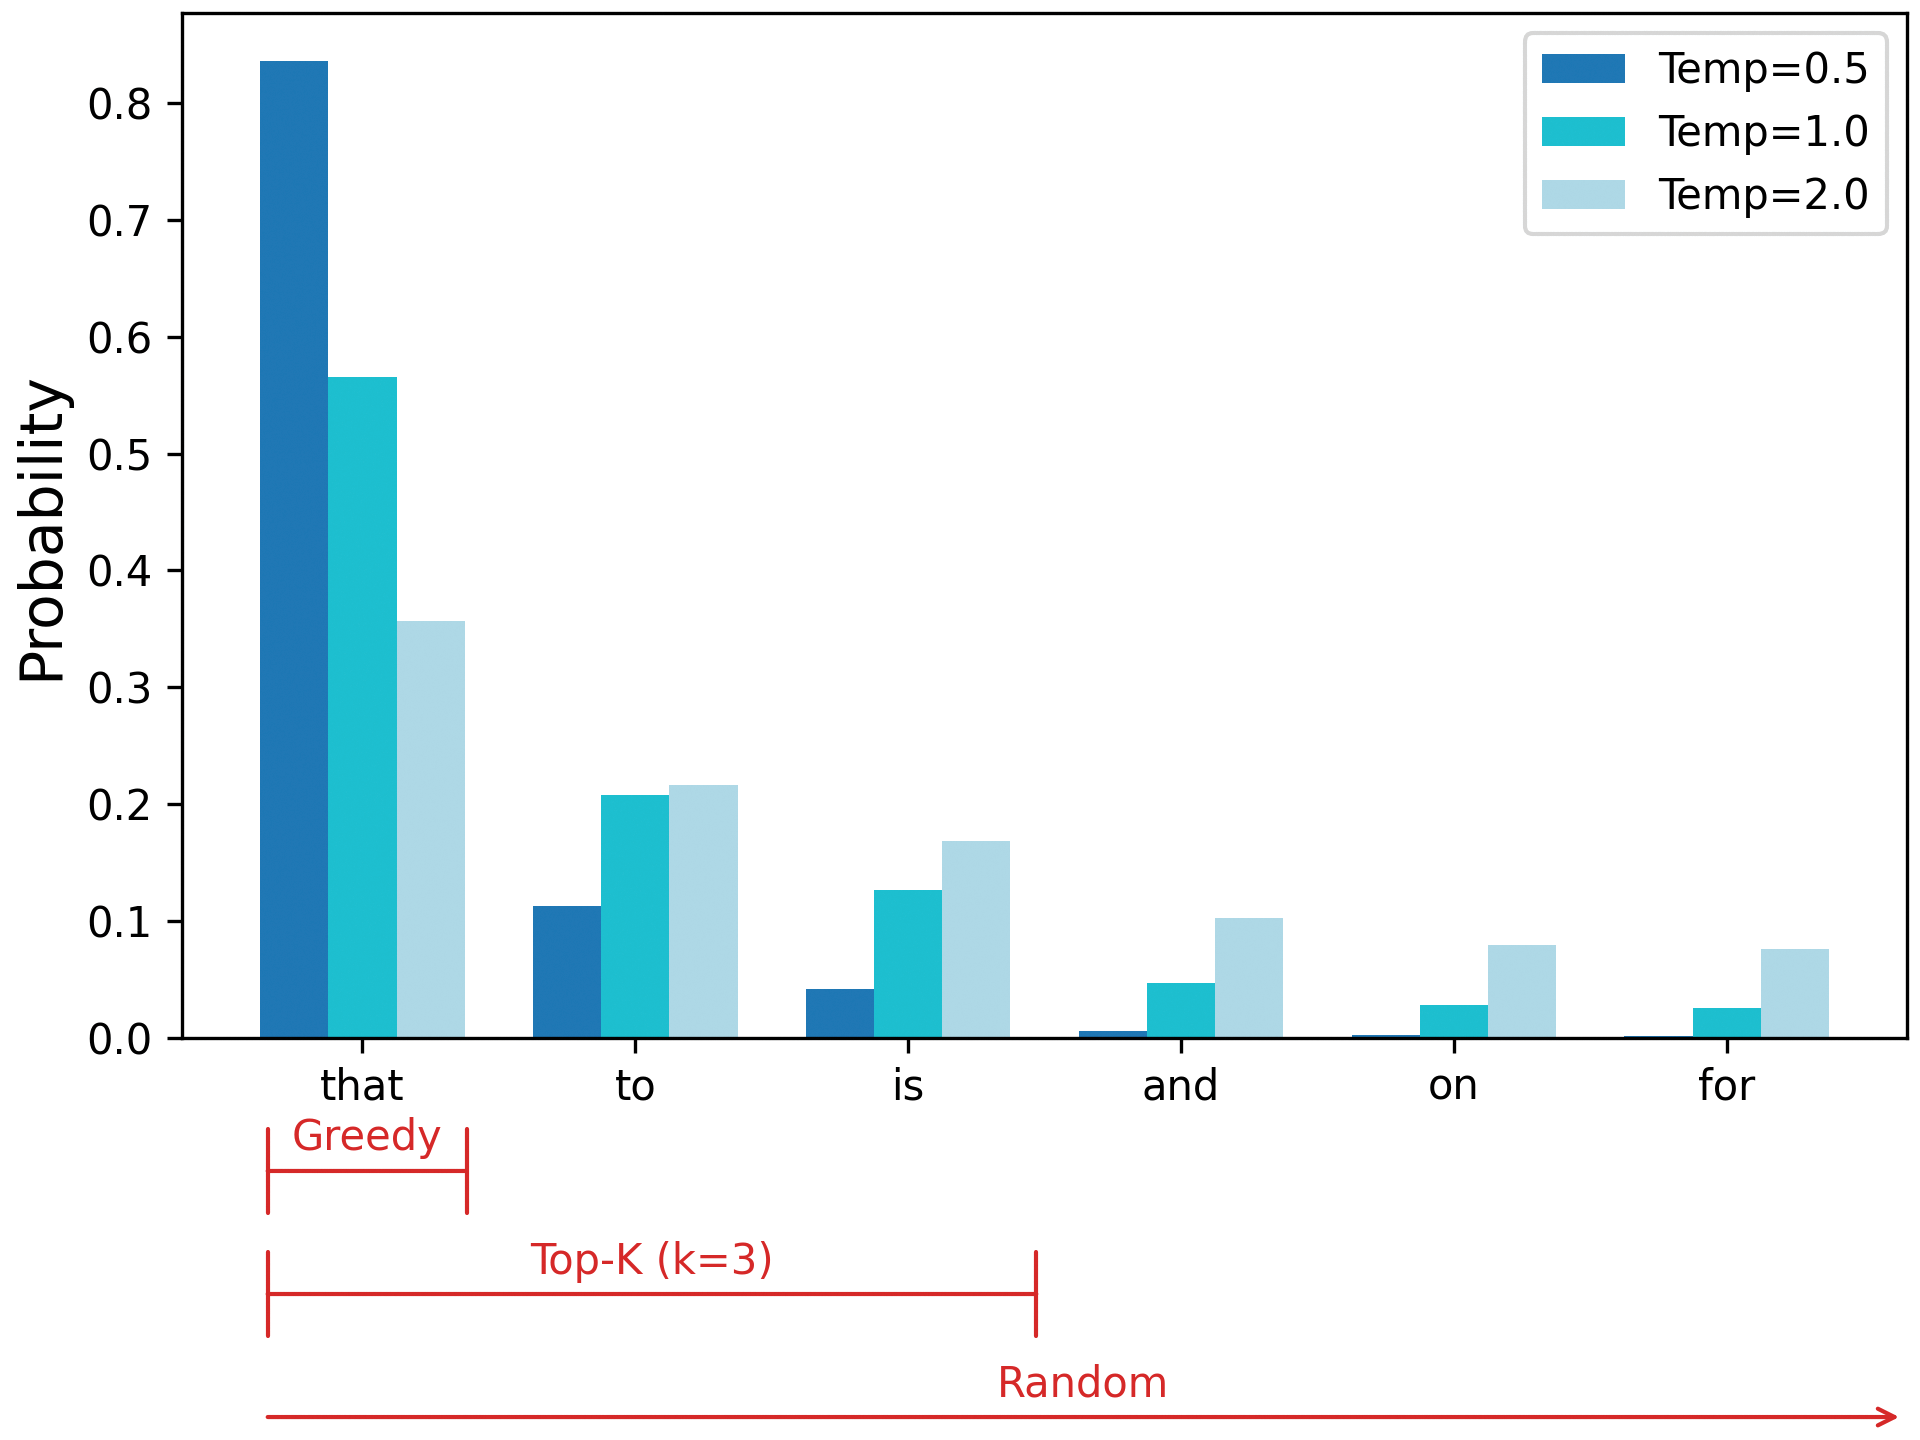
\includegraphics[width=\textwidth,height=0.6\textheight,keepaspectratio]{../../images/ch16/sampling-strategies.0545bedf.png}
            \caption{Cơ chế chặn lọc của Top-K và Top-p}
        \end{figure}
    \end{columns}
\end{frame}

\section{4. Tinh chỉnh và Sử dụng LLM}

\begin{frame}{Sử dụng LLM đã được đào tạo trước (Pre-trained LLM)}
    \begin{itemize}
        \item Huấn luyện GPT từ đầu cực kỳ tốn kém và tiêu thụ năng lượng khổng lồ, gây ô nhiễm môi trường.
        \item Các mô hình nguồn mở (Llama, Gemma) cho phép cộng đồng dùng chung mô hình đã được huấn luyện trước trên hàng nghìn tỷ token.
        \item Mô hình gốc (Base model) đóng vai trò như một tính năng "Tự động hoàn thành" (Autocomplete) mạnh mẽ, nhưng chưa biết trò chuyện hay làm theo lệnh.
    \end{itemize}
\end{frame}

\begin{frame}{Hướng dẫn tinh chỉnh (Instruction Fine-Tuning)}
    \begin{itemize}
        \item Để biến Base LLM thành Chatbot, ta cần tinh chỉnh nó bằng các tập dữ liệu \textbf{Lệnh - Phản hồi (Instruction - Response)}.
        \item Kết hợp lệnh và phản hồi thành một chuỗi với các token đánh dấu (VD: \texttt{<start\_of\_turn>user ... <end\_of\_turn>}).
        \item Quá trình này dùng Loss Function thông thường (đoán từ tiếp theo) trên đoạn phản hồi.
        \item Mô hình dần thay đổi âm sắc và cách hành xử để trở thành trợ lý AI.
    \end{itemize}
\end{frame}

\begin{frame}[fragile]{Mã nguồn: Fine-Tuning CausalLM}
\begin{lstlisting}[language=Python]
# Compile the pre-trained LLM for fine-tuning
gemma_lm.compile(
    loss=keras.losses.SparseCategoricalCrossentropy(from_logits=True),
    optimizer=keras.optimizers.Adam(5e-5),
    weighted_metrics=[keras.metrics.SparseCategoricalAccuracy()],
)

# Train on instruction-response dataset
gemma_lm.fit(train_ds, validation_data=val_ds, epochs=1)
\end{lstlisting}
\end{frame}

\begin{frame}{Vấn đề VRAM của Fine-Tuning LLM}
    \begin{itemize}
        \item Huấn luyện lại một mô hình LLM vài tỷ tham số đòi hỏi lượng RAM GPU khổng lồ.
        \item Trình tối ưu hóa (Optimizer) như Adam lưu giữ thêm 3 trạng thái cho mỗi tham số (Gradient, Velocity, Momentum).
        \item Tổng cộng bộ nhớ yêu cầu phình to gấp 3-4 lần số tham số gốc. GPU phổ thông 16GB sẽ gặp lỗi \textbf{Out Of Memory (OOM)} ngay bước đầu tiên.
    \end{itemize}
\end{frame}

\begin{frame}{Giải pháp Đại số Tuyến tính: LoRA (Low-Rank Adaptation)}
    \begin{columns}
        \column{0.5\textwidth}
        \begin{itemize}
            \item Ý tưởng cốt lõi: Đóng băng (Freeze) toàn bộ trọng số gốc $W_0$ của mô hình.
            \item Cập nhật thêm một ma trận tinh chỉnh $\Delta W$ bằng cách phân rã thứ hạng thấp (Low-Rank Decomposition) thành tích của ma trận $A$ và $B$.
            \item Hạng $r$ được chọn rất nhỏ (VD: $r=8$).
            $$ W_{\text{mới}} = W_0 + (A \times B) $$
        \end{itemize}
        
        \column{0.5\textwidth}
        \begin{figure}
            \centering
            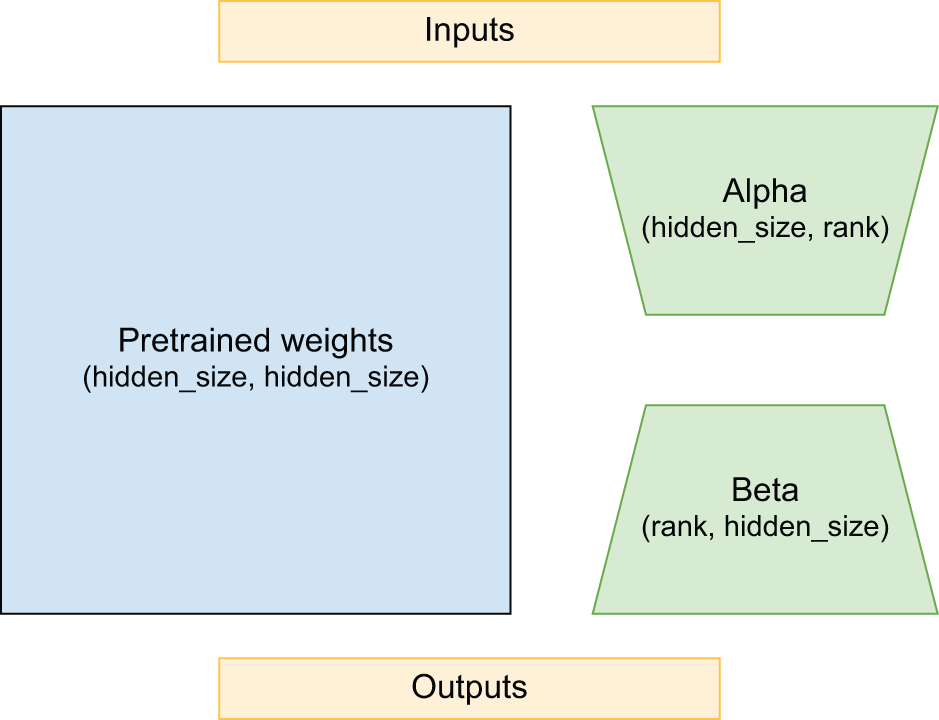
\includegraphics[width=\textwidth,height=0.5\textheight,keepaspectratio]{../../images/ch16/lora-layer.b3119596.png}
            \caption{Cơ cấu ma trận A và B của Lớp LoRA}
        \end{figure}
    \end{columns}
\end{frame}

\begin{frame}{Sự hiệu quả đáng kinh ngạc của LoRA}
    \begin{columns}
        \column{0.5\textwidth}
        \begin{itemize}
            \item Số lượng tham số cần Train giảm xuống cực kỳ khủng khiếp (hơn 1000 lần).
            \item VD: Thay vì update 1 Tỷ tham số (3.7 GB), ta chỉ cần update 5 Megabyte.
            \item Giảm trạng thái lưu trữ của Optimizer, giúp mô hình LLM chạy mượt mà trên các GPU dân dụng.
            \item Hiệu năng (Độ thông minh) của LoRA gần như tương đương Fine-tune toàn phần.
        \end{itemize}
        
        \column{0.5\textwidth}
        \begin{figure}
            \centering
            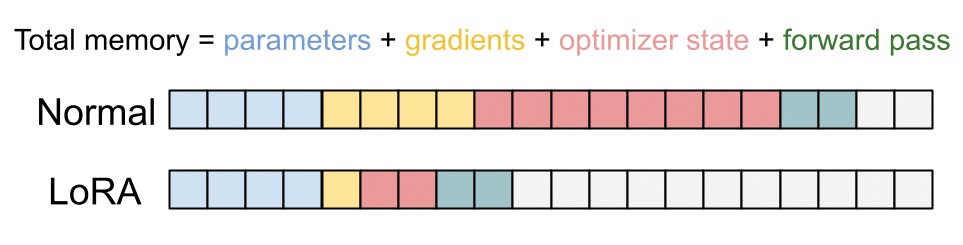
\includegraphics[width=\textwidth,height=0.6\textheight,keepaspectratio]{../../images/ch16/lora-memory.c02fdac4.png}
            \caption{LoRA tiết kiệm tối đa VRAM GPU}
        \end{figure}
    \end{columns}
\end{frame}

\begin{frame}{Học tập tăng cường từ Phản hồi Con người (RLHF)}
    \begin{itemize}
        \item Instruction Fine-tuning (Supervised) bị giới hạn bởi lượng dữ liệu con người viết bằng tay rất đắt đỏ và chậm chạp.
        \item \textbf{RLHF:} Lấy nhiều câu trả lời do AI sinh ra, cho người đánh giá (Human raters) xếp hạng độ ưu tiên từ tốt nhất đến tệ nhất.
        \item Từ dữ liệu xếp hạng đó, hệ thống huấn luyện một \textbf{Mô hình Phần thưởng (Reward Model)} hoạt động thay cho người đánh giá.
    \end{itemize}
\end{frame}

\begin{frame}{Quy trình hoạt động của RLHF}
    \begin{itemize}
        \item \textbf{Agent (LLM)} sinh ra câu trả lời cho một Prompt tùy ý.
        \item \textbf{Environment (Reward Model)} chấm điểm phản hồi đó.
        \item Thông qua thuật toán học tăng cường (như PPO), cập nhật tham số LLM để tối đa hóa phần thưởng.
        \item Phương pháp này giúp mô hình LLM vượt qua giới hạn của Supervised Learning, tạo ra phản hồi thân thiện và an toàn, giống ChatGPT hiện tại.
    \end{itemize}
\end{frame}

\section{5. Tiền phương của LLMs}

\begin{frame}{Tiến hóa thành Mô hình Đa phương thức (Multimodal)}
    \begin{columns}
        \column{0.5\textwidth}
        \begin{itemize}
            \item LLM không chỉ giới hạn ở Văn bản (Text). Bằng cách kết hợp một \textbf{Vision Encoder} (như ViT), ta có \textbf{Vision-Language Model (VLM)}.
            \item Ảnh được cắt thành các bản vá (Patches) và nhúng thành chuỗi vector (Soft tokens) ghép chung vào chuỗi text.
            \item AI giờ đây không chỉ biết đọc chữ, mà còn biết "Nhìn" và hiểu hình ảnh.
        \end{itemize}
        
        \column{0.5\textwidth}
        \begin{figure}
            \centering
            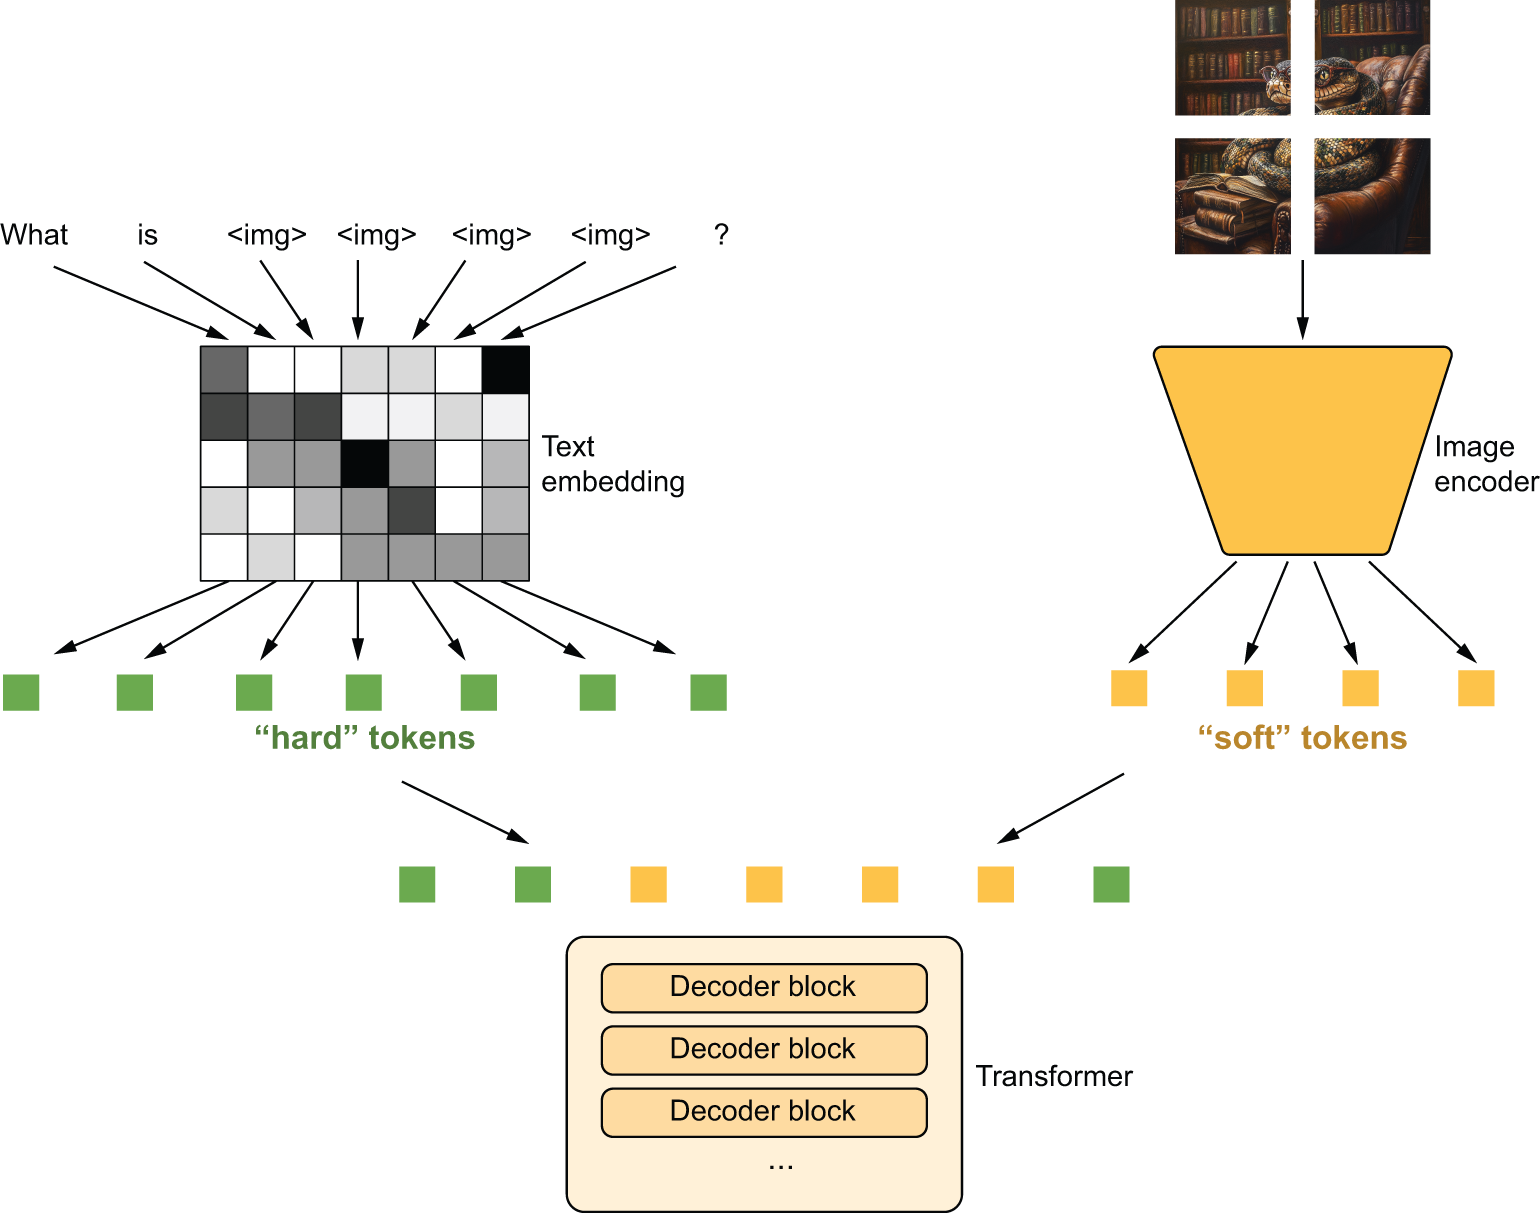
\includegraphics[width=\textwidth,height=0.6\textheight,keepaspectratio]{../../images/ch16/multimodal-transformer.974dc2ec.png}
            \caption{Kiến trúc Multimodal Transformer}
        \end{figure}
    \end{columns}
\end{frame}

\begin{frame}{Thực nghiệm với Mô hình Đa phương thức}
    \begin{columns}
        \column{0.5\textwidth}
        \begin{itemize}
            \item \textbf{Soft Tokens:} Khác với token văn bản cố định, token hình ảnh chứa giá trị vector liên tục trích xuất từ mô hình Computer Vision.
            \item Mô hình VLM có thể mô tả bức ảnh chi tiết: "Một con rắn đeo kính ngồi trên ghế bành đọc sách." hay xác định đối tượng theo yêu cầu.
        \end{itemize}
        
        \column{0.5\textwidth}
        \begin{figure}
            \centering
            \includegraphics[width=\textwidth,height=0.6\textheight,keepaspectratio]{../../images/ch16/gemma-test-image.ddb3b630.png}
            \caption{AI tự động nhận diện và miêu tả hình ảnh}
        \end{figure}
    \end{columns}
\end{frame}

\begin{frame}{Mô hình Nền tảng (Foundation Models)}
    \begin{itemize}
        \item Từ "Large Language Models" không còn đủ ý nghĩa. Các mô hình hiện tại xử lý đồng thời hình ảnh, âm thanh, video, dữ liệu cấu trúc.
        \item \textbf{Foundation Models} là thuật ngữ chung chỉ các mô hình khổng lồ đào tạo trên dữ liệu hỗn hợp toàn cầu bằng Học tự giám sát (Self-supervision).
        \item Cách tiếp cận mới: Thay vì huấn luyện Model từ đầu cho từng bài toán nhỏ, ta dùng Foundation Model làm trung tâm, sau đó tinh chỉnh xuống.
    \end{itemize}
\end{frame}

\begin{frame}{Retrieval-Augmented Generation (RAG)}
    \begin{itemize}
        \item \textbf{Nhược điểm chí mạng của LLM:} Hay bị "Ảo giác" (Hallucination) (bịa đặt thông tin) và kiến thức bị giới hạn tới ngày huấn luyện cuối cùng.
        \item \textbf{RAG (Truy xuất thế hệ tăng cường):} Giải pháp kết nối LLM với Cơ sở dữ liệu Vector (Vector Database) nội bộ hoặc công cụ tìm kiếm trực tuyến.
    \end{itemize}
\end{frame}

\begin{frame}{Cơ chế hoạt động của RAG}
    \begin{itemize}
        \item Khi người dùng đặt câu hỏi, hệ thống RAG trích xuất các tài liệu/văn bản liên quan nhất từ Vector Database.
        \item Ghép nội dung tài liệu đó trực tiếp vào Prompt (Context).
        \item LLM đọc ngữ cảnh đó và \textbf{tổng hợp câu trả lời dựa trên tài liệu thật}, loại bỏ tình trạng AI "bịa chuyện" và cho phép AI tra cứu dữ liệu mới.
    \end{itemize}
\end{frame}

\begin{frame}{Các mô hình Lý luận (Reasoning Models)}
    \begin{itemize}
        \item Các LLM đời đầu rất kém các bài toán Toán học và Logic.
        \item \textbf{Chain-of-Thought (CoT):} Yêu cầu mô hình "Suy nghĩ từng bước" (Step-by-step). Mô hình sẽ viết ra các nháp trung gian để xử lý bài toán hiệu quả hơn.
        \item \textbf{Hiện tại:} Các mô hình mới (OpenAI o1, DeepSeek r1) được huấn luyện để tự động tạo ra một luồng suy nghĩ dài trong tiềm thức (Internal thinking), tự kiểm tra chéo (self-correction) trước khi trả lời.
    \end{itemize}
\end{frame}

\begin{frame}{Tương lai của LLM}
    \begin{itemize}
        \item Mô hình lớn hơn chưa chắc đã thông minh hơn nếu chất lượng dữ liệu huấn luyện thấp. Xu hướng: \textbf{Data-centric AI}.
        \item \textbf{Cạn kiệt dữ liệu (Data Exhaustion):} Nguồn văn bản chất lượng cao trên Internet do con người viết sắp cạn kiệt.
        \item Nếu AI phải học lại từ dữ liệu "rác" do AI sinh ra trên Web, sẽ dẫn đến hiện tượng sụp đổ mô hình (Model Collapse).
    \end{itemize}
\end{frame}

\begin{frame}{Tổng kết Chương 16}
    \begin{itemize}
        \item \textbf{Large Language Models (LLMs):} Sự trỗi dậy mạnh mẽ nhờ Kiến trúc Transformer Decoder-only và Tự giám sát (Unsupervised Pretraining).
        \item \textbf{Sampling \& Fine-tuning:} Nhiệt độ/Top-K tạo sự đa dạng, trong khi Instruction Fine-Tuning và RLHF kiểm soát hành vi và sự an toàn.
        \item \textbf{LoRA:} Đột phá trong việc tối ưu hóa VRAM, cho phép cá nhân hóa mô hình Tỷ tham số bằng GPU phổ thông.
        \item \textbf{RAG \& Multimodal:} Tích hợp CSDL để chống ảo giác và mở rộng mô hình sang chiều không gian đa phương thức.
    \end{itemize}
\end{frame}

\end{document}
